\documentclass[letterpaper,twocolumn,10pt]{article}
\usepackage{usenix-2020-09}
\usepackage{amsmath,amssymb}
\usepackage{booktabs}
\usepackage{graphicx}
\usepackage{xcolor}
\usepackage{enumitem}
\usepackage{balance}
\usepackage{url}
\usepackage{microtype}
\usepackage{xspace}
\usepackage{float}
\usepackage{etoolbox}

\graphicspath{{img/}}
\setlist{leftmargin=*,nosep}
% Keep the two-column layout dense, matching the compact OSDI style.
\setlength{\parskip}{0pt}
\setlength{\textfloatsep}{1pt plus .5pt minus .5pt}
\setlength{\floatsep}{1pt plus .5pt minus .5pt}
\setlength{\intextsep}{2pt plus .5pt minus .5pt}
\setlength{\abovecaptionskip}{1pt}
\setlength{\belowcaptionskip}{0pt}
\setlength{\abovedisplayskip}{2pt plus .5pt minus .5pt}
\setlength{\belowdisplayskip}{2pt plus .5pt minus .5pt}
\setlength{\abovedisplayshortskip}{.5pt plus .5pt minus .5pt}
\setlength{\belowdisplayshortskip}{.5pt plus .5pt minus .5pt}
\makeatletter
\renewcommand\section{\@startsection {section}{1}{\z@}{-2.8ex plus-.8ex minus-.2ex}{.6ex plus.1ex}{\reset@font\large\bfseries}}
\renewcommand\subsection{\@startsection{subsection}{2}{\z@}{-2.1ex plus-.6ex minus-.2ex}{.3ex plus.1ex}{\reset@font\normalsize\bfseries}}
\renewcommand\subsubsection{\@startsection{subsubsection}{3}{\z@}{-1.6ex plus-.4ex minus-.1ex}{.15ex plus.1ex}{\reset@font\normalsize\bfseries}}
\renewcommand\paragraph{\@startsection{paragraph}{4}{\z@}{-1.1ex plus-.3ex minus-.1ex}{0pt plus.1ex}{\reset@font\normalsize\bfseries}}
\makeatother
\newcommand{\system}{\textsc{AgentTX}\xspace}
\newcommand{\aet}{\textsc{AET}\xspace}
\newcommand{\trycmd}{\texttt{try}\xspace}
\AtBeginEnvironment{thebibliography}{%
  \normalsize
  \setlength{\itemsep}{-0.2pt}
  \setlength{\parsep}{0pt}
  \setlength{\parskip}{0pt}}

\begin{document}
\date{}
\title{\Large \bf \system: Causal Effect Transactions for Long-Running Coding Agents}
\author{Anonymous submission}
\maketitle

\begin{abstract}
Coding agents increasingly execute long, stateful trajectories in which later
tool calls reuse filesystem state produced by earlier editing, compilation, and
testing. Existing speculative execution mechanisms preserve and recover state at
command, session, branch, or checkpoint boundaries. We observe that these
boundaries create a granularity mismatch: short-lived isolation repeatedly
reconstructs execution state, while coarse temporal recovery can discard later
work that is independent of a failed step. We present \system, which decouples
the speculation unit from the recovery unit. A trajectory executes in one
continuous speculative workspace, while recovery selects only filesystem effects
that causally depend on a failed step. \system uses Agent Effect Transactions
(\aet) as its causal recovery module and combines dependency capture,
object-aware reconstruction, and durable publication. Across 144 controlled
runs, \system retained 100\% of independent work and removed 100\% of invalid
descendants; temporal recovery retained only 41\% of independent work at
64 calls. At 48 document entries, preserving valid later work avoided 1,425
replay tokens relative to temporal recovery and 3,340 relative to whole-session
abort.
\end{abstract}


\section{Introduction}

Coding agents increasingly solve software-engineering tasks through long
sequences of interactions with a development environment rather than producing
a patch in a single turn. Their control loops interleave model reasoning with
tool actions and observations, allowing plans to change after commands fail or
reveal new repository evidence~\cite{react}. Systems such as SWE-agent and
OpenHands expose repository navigation, file editing, shell commands, and tests
to the model~\cite{sweagent,openhands}, while SWE-bench evaluates issue
resolution as an interactive process spanning multiple files and test
runs~\cite{swebench}. Consequently, the filesystem becomes persistent execution
state: later compilation, testing, and repair steps can directly consume files
and artifacts produced earlier in the same trajectory.

Existing systems preserve this evolving state at different boundaries.
Command-level semisolates such as \trycmd stage one opaque invocation and expose
its effects before application~\cite{try-osdi26}; agent-facing filesystems and
branch runtimes preserve longer-lived workspace state~\cite{yolofs,branchfs};
and checkpoint systems restore an earlier temporal execution state
~\cite{waypoint,deltabox}. Process checkpointing provides related restart
guarantees~\cite{criu,dmtcp}; transactional filesystems provide related
publication guarantees~\cite{valor,txfs}.
Although these systems differ in purpose and implementation, their native
recovery unit largely follows the state unit they preserve: a command, branch,
session, checkpoint, or transaction. Our study reveals a tension in this design.
Short-lived isolation repeatedly reconstructs execution state along a long
trajectory, whereas longer-lived sessions and checkpoints preserve state but
recover it at a coarser temporal granularity.

This tension becomes important because temporal order does not imply failure
dependence. Consider four interleaved steps: $s_0$ writes a faulty formatter,
$s_1$ reads it and generates a report, $s_2$ edits an unrelated document, and
$s_3$ tests the faulty output. Recovery should remove
$\{s_0,s_1,s_3\}$ while retaining $s_2$. Undoing only $s_0$ leaves derived
state behind, whereas rolling back the suffix from $s_0$ also discards the
independent edit. Our motivational experiments show the same mismatch at
larger scale: checkpoint-style temporal recovery retained only 41\% of
independent work at 64 calls, while whole-session recovery retained none.
These observations suggest that the lifetime of speculation and the granularity
of recovery are different system concerns: long-running agents benefit from a
large speculation unit, but failure recovery may require a non-contiguous
subset of that unit.

Recovering such a subset raises three systems challenges: 1) \emph{dependency
discovery} must identify producer--consumer relations hidden behind shells,
compilers, tests, and descendant processes; 2) \emph{object identity} must
relate effects across aliases, renames, replacements, and copy-up, where
pathname equality may not imply object equivalence; and 3) \emph{selective
reconstruction} must remove dependent effects while preserving later
independent versions rather than restoring an earlier snapshot wholesale.
To address these challenges, we present \system, which separates the
\emph{speculation unit} from the \emph{recovery unit}. An agent trajectory
executes in one continuous speculative workspace, while recovery operates over
dependencies among versioned filesystem effects. At the core of \system,
Agent Effect Transactions (\aet) record observed filesystem effects and their
causal relations to identify the subset affected by a failure. \system then
reconstructs the corresponding object versions, preserves independent later
state, and publishes only approved effects to the host.

We implemented \system on Linux with dependency capture, object-aware
historical reconstruction, fail-closed alias handling, and durable
publication. Across 144 controlled runs, \system retained 100\% of independent
work while removing 100\% of invalid descendants. At 64 calls, temporal
recovery retained only 41\% of independent work. At 48 document entries,
preserving valid artifacts avoided 1,425 replay tokens relative to temporal
recovery and 3,340 relative to whole-session abort. These results indicate that
recovery granularity is not only an execution-overhead problem: reducing
isolation cost cannot recover valid work once a coarse rollback boundary has
discarded it.

This paper makes four contributions:
\begin{itemize}
  \item We analyze existing speculation and recovery boundaries for multi-step
        coding agents and identify a mismatch between long-lived speculative
        execution and selective failure recovery.

  \item We design \system to separate the speculation unit from the recovery
        unit, allowing a continuous workspace to recover non-contiguous
        dependent effects while retaining later independent work.

  \item We introduce \aet as the causal recovery module in \system and realize
        it with dependency capture, versioned object identity, selective
        reconstruction, and durable publication.

  \item We evaluate \system through controlled recovery, runtime, replay-token,
        identity, failure-recovery, and concurrency experiments.
\end{itemize}


\section{Background}
\label{sec:background}

\subsection{Stateful Coding-Agent Workspaces}

Coding agents execute software-engineering tasks as iterative interactions with
an operating-system environment.  Systems such as SWE-agent and OpenHands let a
model inspect repositories, edit files, invoke shell commands, and run tests
~\cite{sweagent,openhands}.  A task therefore spans multiple tool calls rather
than one isolated program execution.  Each call observes the repository state
left by earlier calls, and shells can launch compilers, test runners, package
managers, and other descendant processes whose effects become part of the same
workspace.  The filesystem is consequently persistent execution state for the
agent: source edits, generated artifacts, build products, and configuration
changes can be consumed by later calls in the same session.

The broader agent literature makes this execution pattern explicit.  Tool-use
controllers learn when to invoke external APIs~\cite{toolformer}.  Reasoning-
and-action loops and self-reflection extend trajectories across feedback
steps~\cite{reflexion}.  Interactive benchmarks evaluate multi-turn state and
real websites, as in AgentBench~\cite{agentbench} and WebArena~\cite{webarena}.
Desktop and stateful-tool suites broaden this setting to OSWorld~\cite{osworld}
and ToolSandbox~\cite{toolsandbox}; AppWorld evaluates longer application
workflows~\cite{appworld}, while BrowserGym targets multi-step web interaction
~\cite{browsergym}.

This execution model makes the workspace boundary important.  Direct execution
exposes every mutation to the host as soon as a tool runs.  Recent agent systems
instead keep filesystem changes provisional.  YoloFS stages session mutations
outside the base filesystem and provides snapshots that an agent can return to
during self-correction~\cite{yolofs}.  OpenHands similarly supports sandboxed
execution for software-development agents~\cite{openhands}.  These systems let
an agent continue operating on a mutable workspace while delaying or
controlling when its effects become durable.

Repository-level coding systems add another source of long-lived state.  They
retrieve context across files, localize faults, edit repositories, and execute
tests iteratively; RepoCoder~\cite{repocoder} and AutoCodeRover
~\cite{autocoderover} illustrate this workflow.  Agentless and HyperAgent
extend it to autonomous repair~\cite{agentless,hyperagent}, while SWE-gym
studies longer interactive trajectories~\cite{swegym}.  Recent benchmarks
broaden the workload from issue fixes to feature development and software
evolution~\cite{sweevo}.  FeatureBench studies feature-level development
~\cite{featurebench}, while SWE-rebench revisits repository evolution
~\cite{swerebench}.  Other suites cover repository-scale work, research
replication, and experiment execution; examples include GitTaskBench
~\cite{gittaskbench}, PaperBench~\cite{paperbench}, and MLAgentBench
~\cite{mlagentbench}.

\subsection{Speculation and Recovery Units}

Systems that keep execution provisional differ primarily in the state unit they
preserve and later recover.  \trycmd introduces a semisolate around an opaque
component invocation: it captures the command's filesystem effects so they can
be inspected, applied, stacked, or discarded before they modify the live
system~\cite{try-osdi26}.  Agent-native filesystems extend this lifetime across
a session.  YoloFS retains staged mutations and uses snapshots as restoration
points~\cite{yolofs}, while BranchFS gives each speculative branch an isolated
copy-on-write filesystem view with branch-level commit or abort
~\cite{branchfs}.

Checkpoint/restore systems preserve still broader execution state.  Crab
observes turn-level OS effects to decide when a sandbox checkpoint is
recovery-relevant, but restoration still returns the sandbox to a selected
checkpoint~\cite{crab}.  DeltaBox accelerates checkpoint and rollback of
stateful agent sandboxes by storing changes between consecutive checkpoints;
its restored state includes both filesystem and process state
~\cite{deltabox}.  Thus, these systems span command effects, staged sessions,
branches, and complete sandbox checkpoints.  Table~\ref{tab:granularity}
summarizes the corresponding speculative and recovery boundaries.

\begin{table}[H]
\centering
\scriptsize
\setlength{\tabcolsep}{5pt}
\renewcommand{\arraystretch}{1.10}
\caption{\textbf{Speculative state and native recovery boundaries.}
Existing agent execution substrates preserve state at command, session,
branch, or checkpoint granularity.}
\resizebox{0.8\columnwidth}{!}{%
\begin{tabular}{@{}lll@{}}
\toprule
System & Speculative state & Recovery boundary \\
\midrule
\trycmd~\cite{try-osdi26}
  & Opaque-command effects
  & Command effect set \\
YoloFS~\cite{yolofs}
  & Staged session
  & Snapshot \\
BranchFS~\cite{branchfs}
  & Branch context
  & Branch \\
Crab~\cite{crab}
  & Sandbox state
  & Checkpoint \\
DeltaBox~\cite{deltabox}
  & Sandbox state
  & Checkpoint \\
\bottomrule
\end{tabular}%
}

\label{tab:granularity}
\end{table}


As Table~\ref{tab:granularity} shows, the lifetime of speculative execution and
the boundary exposed for recovery are defined by each substrate's state
abstraction.  Command-level effect capture provides a short-lived boundary,
whereas staged filesystems, branches, and checkpoints preserve progressively
longer-lived execution state.  These abstractions provide the execution
substrates for the recovery behaviors examined next.

\section{Observation and Motivation}
\label{sec:motivation}

\subsection{Isolation Overhead Overview}

With stateful agent execution and speculative workspaces in place, one question
arises: how much overhead is introduced when isolation is repeatedly established
along a long tool-call trajectory?  We examine the execution path before
turning to recovery semantics.

\textbf{Methodology.}
We run an isolation microbenchmark under execution modes that
approximate the systems in Table~\ref{tab:granularity}, plus unsafe bare
execution.  Trajectory length varies over equal steps $32,64,96,128$ tool
calls, mixing shell, read, write, compile, and filesystem listing work.
Application evaluation in Section~\ref{sec:eval} uses only SWE-Bench Lite and
Terminal-Bench.  We
measure end-to-end wall time per tool call, host cleanliness before approval,
and the p50/p95 tails.

\textbf{Observation \#1: Rebuilding isolation at tool boundaries incurs
substantial repeated cost.}
Figure~\ref{fig:motivation-scaling} compares the systems in
Table~\ref{tab:granularity} across equal-step lengths $32,64,96,128$.  Bare
execution provides a latency lower bound (8.4~ms/step at 64 calls) but mutates
the host immediately.  Per-call \trycmd stays near 1659.9--1684.9~ms/step across
the sweep.  YoloFS/BranchFS proxies that still re-enter a \trycmd overlay each
call track that cost within a few percent.  Checkpoint-oriented floors in the
style of Crab and DeltaBox fall from 127.8--129.6~ms/step at 32 calls to
47.3--47.6~ms/step at 128 calls while keeping the host clean.  The gap indicates
that repeated namespace and overlay setup, rather than the tool workload alone,
is a major cost when isolation is re-established near every tool boundary; longer
trajectories amortize checkpoint-style setup more than overlay setup.  The tail
(Figure~\ref{fig:motivation-tail}) remains dominated by systems that re-establish
isolation near tool boundaries rather than by the bare tool work alone.

\begin{figure}[t]
  \centering
  
\includegraphics[width=0.98\columnwidth]{FIG-Motivation-Scaling.pdf}
  \caption{\textbf{Longer trajectories amortize setup but do not remove
  isolation cost.} \small\emph{Across 32, 64, 96, and 128 calls, checkpoint
  floors amortize fixed setup, while \trycmd-backed YoloFS/BranchFS proxies
  stay near per-call overlay cost. All remain above bare. The end-to-end panel
  shows why per-step latency alone is insufficient for long sessions.}}
  \label{fig:motivation-scaling}
\end{figure}

\begin{figure}[t]
  \centering
  
\includegraphics[width=0.98\columnwidth]{FIG-Motivation-Tail-Scaling.pdf}
  \caption{\textbf{Existing substrates leave different tail profiles.}
  \small\emph{Per-call \trycmd dominates both median and p95 call latency.
  Session/branch staging and checkpoint floors reduce the tail relative to
  \trycmd but remain above bare at every tested length.}}
  \label{fig:motivation-tail}
\end{figure}

\subsection{Recovery Behavior Breakdown}

The previous observation favors a workspace whose lifetime spans multiple tool
calls.  This raises a follow-up question: when one intermediate step is rejected
or fails, what state should a long-lived speculative workspace discard?

\textbf{Methodology.}
We execute real filesystem effect DAGs rather than simulated graph nodes.  The
sweep varies trajectory length (16/32/64), shape (chain, fan-out, layered),
fault position (10/50/75\%), and independent-work ratio (25/50/75\%).  We
compare the recovery styles of existing substrates: checkpoint-style temporal
rollback, session/branch abort, and command undo without dependency tracking.
Results are summarized in Figure~\ref{fig:motivation-recovery}.  Every run
checks both the speculative view and the physical host before commit.

\textbf{Observation \#2: Temporal recovery removes invalid suffix state but
also discards later work that is independent of the failure.}
Figure~\ref{fig:motivation-recovery} evaluates the recovery styles implied by
Table~\ref{tab:granularity} on the same effect-DAG sweep, without introducing
our system.  Checkpoint-style temporal rollback (Crab/DeltaBox) removes the
invalid suffix but retains only 41\% of independent work at 64 calls.
Session/branch abort (YoloFS/BranchFS) retains 0\%.  Command-level undo without
dependency tracking preserves apparent later files but removes only 4\% of
invalid descendants.  In the long workload, the fault roots are steps
$[27,29,30]$; undoing only the producer leaves derived corruption behind, while
suffix/session abort also discards later independent edits.

\begin{figure}[t]
  \centering
  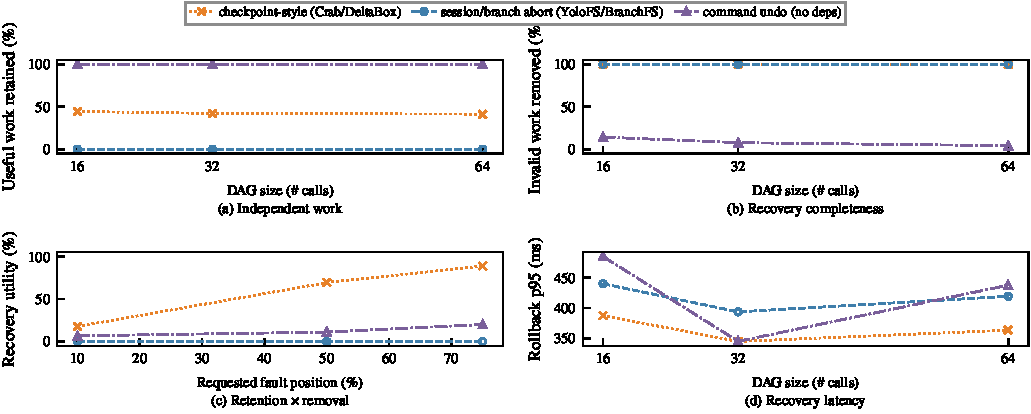
\includegraphics[width=0.98\columnwidth]{FIG-Motivation-Recovery.pdf}
  \caption{\textbf{Existing recovery substrates discard independent work.}
  \small\emph{Checkpoint-style temporal rollback, session/branch abort, and
  dependency-unaware command undo on the controlled effect-DAG sweep
  (16/32/64). AgentTX is omitted. At 64 calls, temporal recovery retains 41\%
  of independent work, session abort retains none, and undo-without-deps
  removes only 4\% of invalid descendants.}}
  \label{fig:motivation-recovery}
\end{figure}

\textbf{Recovery analysis.}
The result comes from a mismatch between execution order and state dependence.
A later step may consume a file produced by a failed step, while another later
step may modify an unrelated file.  Reverting only the failed call leaves the
derived effect behind; reverting the complete suffix removes both effects.
Whole-session recovery widens this boundary further.  The temporal policy
therefore loses 59\% of independent work at 64 calls before any model is asked
to regenerate it.

This loss also appears as additional agent work.  In the controlled token
experiment, retaining valid artifacts avoids 1,424.7 replay tokens relative to
an optimistic temporal checkpoint and 3,340.3 relative to whole-session abort
at 48 document entries.  These numbers measure recovery-induced replay rather
than total session-token savings.  Reducing execution overhead alone cannot
recover work that has already been discarded by the recovery boundary.

\subsection{Recovery Boundaries in Stateful Agent Execution}
\label{sec:recovery-granularity}

\textbf{Existing recovery boundaries.}
The previous observations expose a gap between speculative execution and
recovery granularity. Existing agent execution substrates have explored
different ways to preserve intermediate state. Command-level semisolates
protect the host while executing individual operations, while session, branch,
and checkpoint mechanisms maintain longer-lived execution contexts and restore
state at coarser boundaries. Among these approaches, \trycmd is particularly
relevant to coding agents because it treats a tool invocation as an opaque
execution unit: a command can execute with isolated filesystem effects and
selected results can later be published. We therefore use \trycmd-based
isolation as a representative speculative execution baseline rather than bare
execution, which provides no protection or recovery boundary.

\textbf{Mismatch in state propagation.}
Preserving speculative state and deciding what state to recover are different
problems. A coding-agent trajectory can be viewed as an ordered sequence of
tool calls $T=\langle s_0,s_1,\ldots,s_n\rangle$, where each step executes on
the workspace state produced by earlier steps. Existing mechanisms usually
define recovery according to execution structure: command-level recovery affects
only the current step, session-level recovery discards the whole speculative
workspace, and checkpoint-style recovery removes a temporal suffix beginning
at a selected point. These policies are effective when execution boundaries
closely match state boundaries, but this assumption becomes weak for
long-running agent trajectories.

For example, consider a trajectory where $s_0$ introduces an incorrect code
change, $s_1$ compiles and generates artifacts from that change, $s_2$ edits an
unrelated document, and $s_3$ runs another test that consumes the incorrect
artifact. A session abort or temporal checkpoint rollback removes all later
steps, including the valid edit from $s_2$. In contrast, undoing only $s_0$
leaves artifacts produced by $s_1$ and $s_3$ in the workspace. The desired
recovery state is therefore not determined by execution order alone.

\textbf{Hidden dependencies across execution.}
Determining which later state remains valid is difficult because tool boundaries
do not fully expose how state propagates through execution. A shell command,
compiler, test runner, or descendant process may consume intermediate state and
create new artifacts that are later observed by other steps. The execution
history records when these actions occur, but not necessarily how their effects
influence one another.

\textbf{Object identity beyond path names.}
Filesystem state introduces another source of ambiguity. Paths provide the
interface through which tools access files, but they are not always stable
identifiers for recovery. Aliases, renames, replacements, and layered
filesystems can make different paths refer to related objects or make the same
path represent different versions over time. Recovering part of a trajectory
therefore requires understanding both the propagation of effects and the state
represented by those effects.

\textbf{Implication.}
These observations motivate a recovery abstraction that separates the lifetime
of speculation from the granularity of recovery. A long-running trajectory
should execute in a persistent speculative workspace, while recovery should
remove only the state invalidated by a failure and preserve unrelated later
work. AgentTX follows this separation by using Agent Effect Transactions to
represent filesystem effects and their dependencies.
\section{Agent Effect Transactions}
\label{sec:aet}

The observations in Section~\ref{sec:motivation} expose a mismatch between the
lifetime of an agent trajectory and the unit available for recovery.  AgentTX
addresses this mismatch with an \emph{Agent Effect Transaction} (AET).  An AET
keeps one trajectory speculative, records its versioned effects, recovers a
causal subset, and publishes only an approved frontier.

\subsection{Overview and Design Principles}

\begin{figure}[t]
\centering
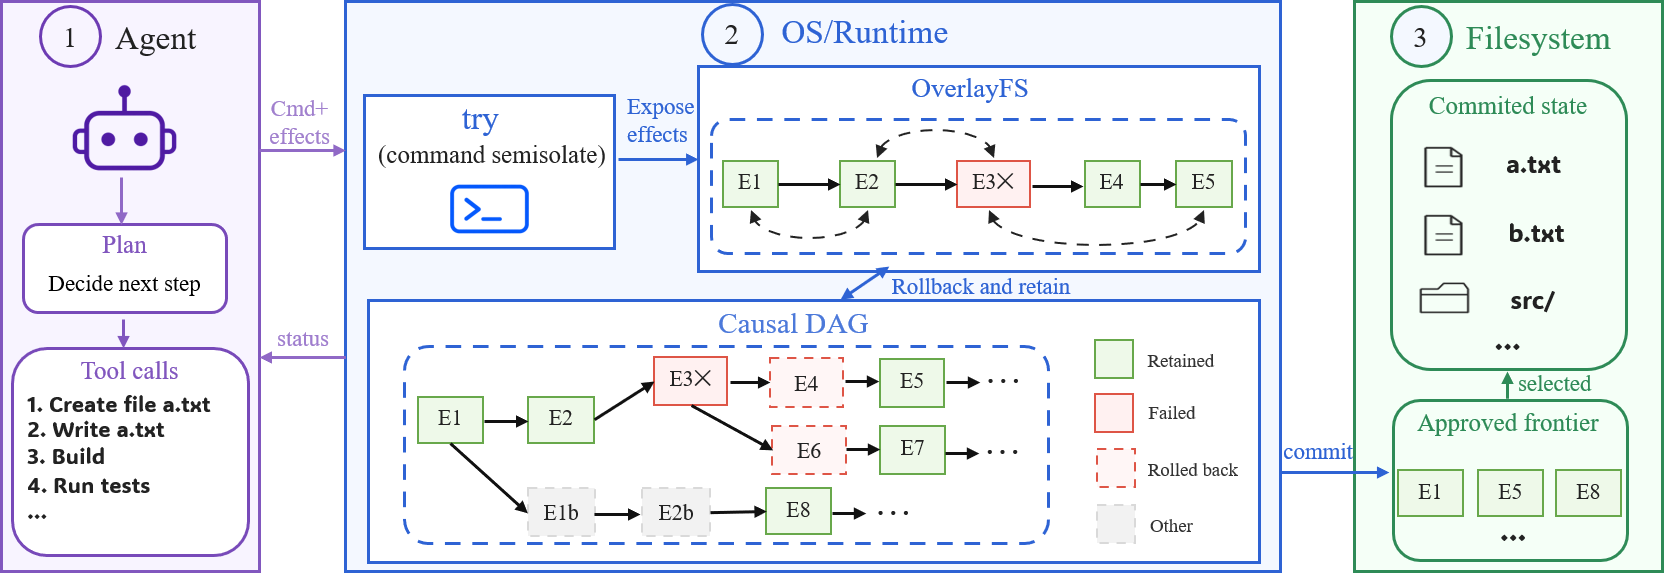
\includegraphics[width=\linewidth]{FIG-AgentTX-Overview.png}
\caption{\textbf{AgentTX separates trajectory-wide speculation from
causal-subset recovery.} \small\emph{Tool calls share one speculative view.
Observed effects form a causal DAG, recovery removes the failed closure, and
only the approved frontier becomes host-visible.}}
\label{fig:overview}
\end{figure}

\textbf{Transaction overview.}
Figure~\ref{fig:overview} follows one trajectory from agent commands to durable
state.  Tool calls execute in a shared speculative view, so each call observes
earlier uncommitted effects.  The host remains unchanged during this execution.

\textbf{Recovery overview.}
Each call contributes typed effects to a ledger.  Producer--consumer edges
connect effects across calls and form a causal DAG.  A failed effect becomes the
root of a transitive closure, while later nodes outside that closure remain
eligible for retention.

\textbf{Publication overview.}
Recovery reconstructs the surviving state before publication.  The runtime
then records an approved frontier and materializes only the versions covered by
that frontier.  A later speculative suffix remains isolated from the host.

\textbf{Design principles.}
The model spans the complete tool-call trajectory rather than one command or
recovery attempt.  It derives causality from observed reads, absence, writes,
and deletes instead of command text; reconstructs object versions that exclude
the failed closure while preserving supported retained effects; and separates
speculative recovery from finalization, the only operation that makes an
approved version host-visible.


\subsection{AET State and Transitions}
\label{sec:aet-model}

\textbf{Scope.}
We model workspace-local filesystem effects produced by trusted but fallible
coding agents.  Network services, process memory, terminal state, and
adversarial confinement remain outside the transaction.

\textbf{State.}
An AET is the tuple $\langle V,L,H,F\rangle$.  $V$ is the current speculative
filesystem view.  $L$ records tool calls, typed
effects, dependencies, and status.  $H$ stores historical object states needed
for reconstruction.  $F$ identifies the boundary approved for publication.

The tuple assigns one role to each correctness concern.  $V$ provides
cross-call state without mutating the host.  $L$ determines causal recovery
sets.  $H$ supplies versions that can remove selected effects.  $F$ separates
approved state from the speculative suffix.

\textbf{Transitions.}
\emph{Append} executes one tool call in $V$ and appends its effects to $L$.
\emph{Recover} computes a causal closure and reconstructs the affected portion
of $V$ from $H$.  \emph{Finalize} advances $F$ and publishes the corresponding
approved versions.

\textbf{Invariants.}
Every successful transition preserves three properties.  \emph{Host isolation}
keeps the host unchanged before finalization.  \emph{Selective recovery}
removes every selected effect while preserving supported, non-overlapping
retained effects.  \emph{Monotonic finalization} prevents a finalized step from
becoming speculative again.

These semantics do not require a particular tracer, snapshot representation,
or publication protocol.  The remaining subsections define the recovery set,
the required historical state, and the approved frontier.


\subsection{Causal Recovery Semantics}
\label{sec:effect-dag}

\textbf{Effect records.}
Each ledger node
$s_i=(i,\mathrm{tool}_i,E_i,P_i,\mathrm{status}_i)$ represents one tool step.
$E_i$ contains its observed filesystem effects and
$P_i$ contains the identifiers of earlier steps on which it depends.  Effects
include successful reads ($R$), negative lookups ($N$), writes ($W$), and
deletes ($D$).

\textbf{Dependency rule.}
Let $\mathrm{overlap}(p,q)$ hold when two effect names identify overlapping
filesystem objects.  For an active earlier step $j<i$, the transaction adds
$j\in P_i$ when:

\begin{itemize}
  \item $s_j$ writes or deletes $p$, and $s_i$ reads, negatively looks up,
        writes, or deletes an overlapping $q$; or
  \item $s_j$ negatively looks up $p$, and $s_i$ later writes an overlapping
        $q$.
\end{itemize}

The write/delete rule captures dependencies induced by observed or subsequently
modified state, including read-after-write and write serialization.  The
negative-lookup rule captures dependencies on absence: a later creation can
invalidate namespace state observed by an earlier negative lookup.

\textbf{Object relation.}
Path equality alone does not define overlap.  We make object identity explicit
with an abstract relation $\equiv_{\mathcal I}$ over effect names.  Path
equality implies overlap, while aliases may also overlap when the identity
relation can establish that they refer to the same object.  A descriptor read
is associated with the object opened earlier only when observation supplies
that relation.  Otherwise, the effect remains unknown instead of receiving a
guessed dependency.  The identity relation is part
of the AET contract; Section~\ref{sec:design} describes how \system
approximates it on Linux.

\textbf{Recovery set.}
For a failed active step $f$, the transitive descendant closure is

\begin{equation}
\begin{aligned}
  C_0(f) &= \{f\},\\[-2pt]
  C_{k+1}(f) &= C_k(f) \cup
    \{s_i \mid P_i \cap C_k(f) \neq \emptyset\},\\[-2pt]
  C(f) &= \bigcup_{k\geq 0} C_k(f).
\end{aligned}
\end{equation}

$C(f)$ is the least transitive descendant closure of $f$ among active,
uncommitted steps.  It may contain steps that are separated in time by
independent work.  Temporal rollback instead selects the contiguous suffix
$\{s_i \mid i\geq f\}$, regardless of whether each later step depends on $f$.


\subsection{Object-Aware Reconstruction}
\label{sec:selective-reconstruction}

\textbf{Target version.}
Computing $C(f)$ identifies which effects should no longer contribute to the
speculative state, but removing their latest writes is not sufficient when the
same object has been modified repeatedly.  Recovery must instead reconstruct
the version that would remain after excluding the selected causal subset.

Let $W(C)$ denote the objects written or deleted by steps in $C(f)$.  For each
target in $W(C)$, recovery obtains from $H$ a historical state that predates its
earliest selected effect.  The retained active history is then considered
against the selected targets so that later independent state is not discarded
solely because it occurs after the failed step.

\textbf{Retained overlap.}
A retained effect can nevertheless conflict with selective reconstruction.  If
a retained active effect overlaps a target in $W(C)$ and the model cannot
establish a supported reconstruction, recovery rejects the operation rather
than guessing a merge.  This fail-closed rule trades availability for the
following safety invariant:

\textbf{Recovery guarantee.}
After a successful causal rollback, no effect written by $C(f)$ remains
visible.  Every non-overlapping retained effect remains visible in the
speculative view.

Only after reconstruction succeeds are the selected ledger nodes marked as
rolled back.  Reconstruction therefore changes the workspace by causal
membership rather than restoring a complete temporal snapshot.  Unreachable
historical states may then be reclaimed.


\subsection{Approved Commit Frontier}
\label{sec:commit-frontier}

\textbf{Frontier semantics.}
Recovery determines which speculative effects remain active; finalization
determines which of those effects become durable.  AET separates these two
operations through the frontier $F$.

$F$ is the largest finalized step identifier.  Every step at or below $F$ is
either approved for publication or durably marked as rolled back.  Advancing
the frontier from $F$ to $F'>F$ publishes active write/delete effects in
$(F,F']$ while leaving later steps speculative.  Rolled-back holes therefore do
not prevent monotonic progress of the frontier.

\textbf{Version selection.}
The version associated with the frontier, rather than the latest speculative
version, determines what is published.  If a later speculative step rewrites
an object whose earlier version has already reached the frontier,
\emph{Finalize} must publish the frontier version without exposing the later
speculative rewrite.

\textbf{Durability boundary.}
Publication and speculative recovery are therefore separate AET transitions.
AET requires the publication transition to be durably recoverable after an
interruption, but does not require atomic multi-path visibility to external
observers.  The concrete durability, version-storage, and publication
mechanisms are implementation choices described
in Section~\ref{sec:design}.

\section{AgentTX Implementation}
\label{sec:design}

AgentTX maps each AET component to a concrete Linux mechanism.  A shared
OverlayFS view realizes $V$, effect capture populates $L$, and the version store
and object catalog provide $H$.  Policy-checked WAL publication advances $F$.
The implementation follows one data path from speculative execution to durable
publication; performance mechanisms are separated at the end of the section.

\subsection{Runtime Architecture and Continuous Speculation}

\begin{figure}[t]
\centering
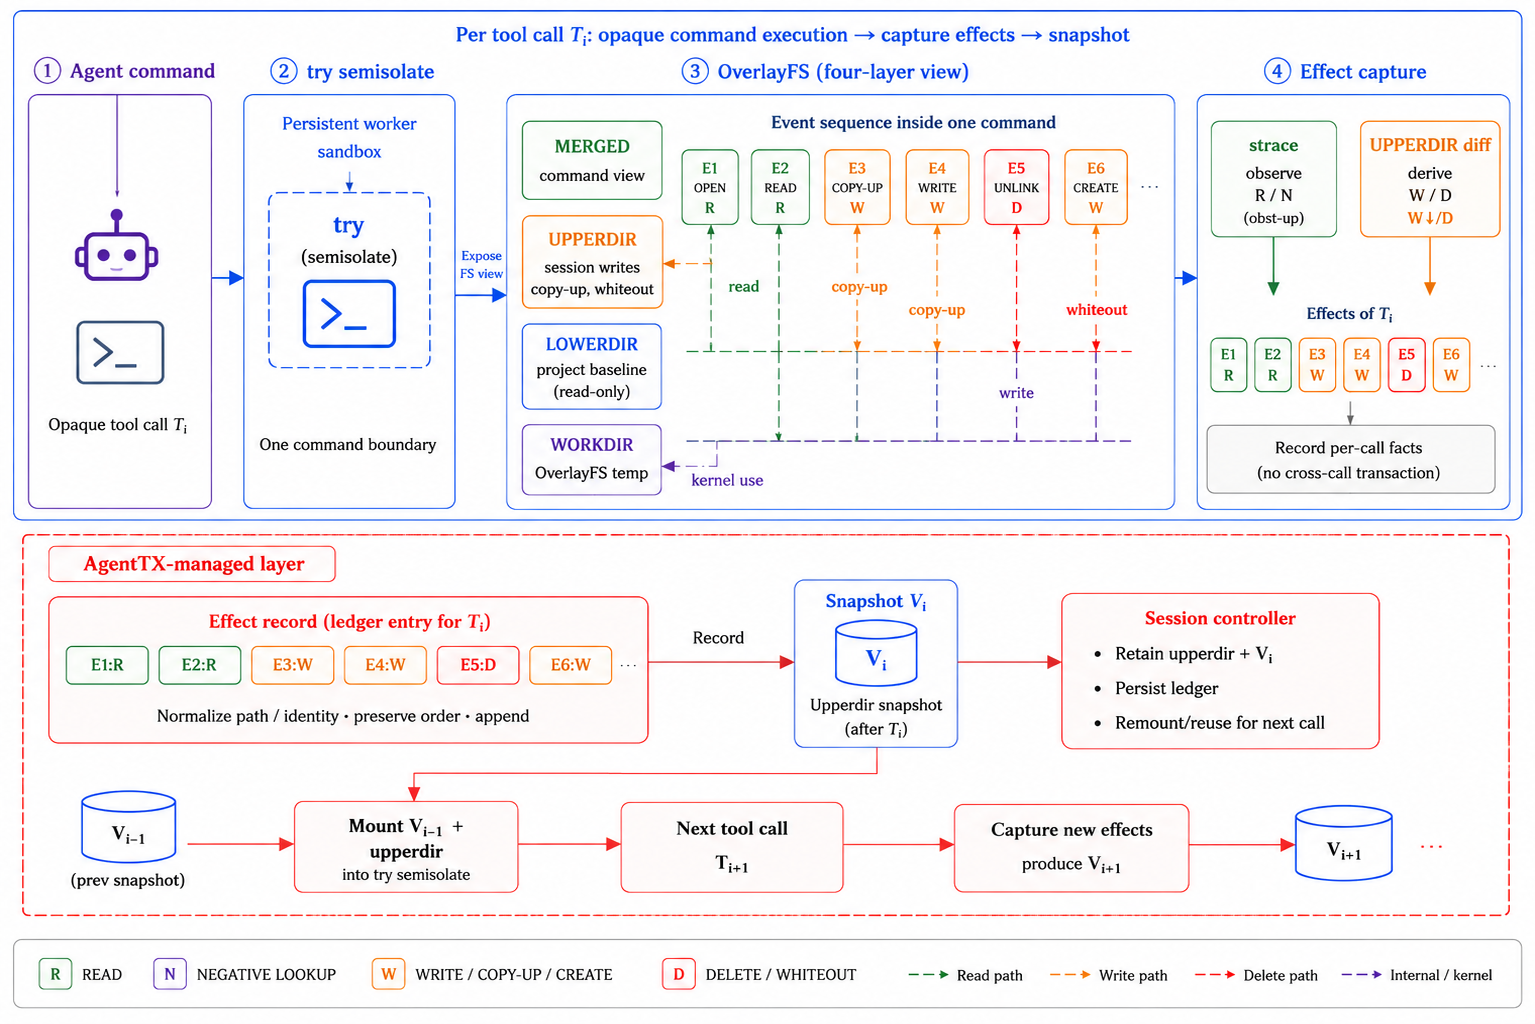
\includegraphics[width=\linewidth]{FIG-Per-Call-Continuous-Speculation.png}
\caption{\textbf{One tool call extends the shared speculative state.}
\small\emph{A call executes in a four-directory OverlayFS view.  Complementary
observers produce typed effects, AgentTX appends record $E_i$, and snapshot
$V_i$ becomes historical input for later recovery.  DAG construction starts
after this per-call record exists.}}
\label{fig:continuous-speculation}
\end{figure}

\textbf{Workspace construction.}
Figure~\ref{fig:continuous-speculation} shows the runtime path for one call
$T_i$.  AgentTX selects the project baseline as the read-only
\texttt{lowerdir}, creates the session's writable \texttt{upperdir}, and
allocates the OverlayFS \texttt{workdir} and \texttt{merged} mount point.  The
command runs against \texttt{merged}, not the host project.

OverlayFS resolves reads against the upper layer and then the baseline.  A
write to a lower object triggers copy-up, a new object enters the upper layer,
and deletion creates a whiteout.  The kernel uses \texttt{workdir} for internal
bookkeeping.  AgentTX configures these directories and controls their lifetime;
OverlayFS performs lookup, copy-up, and whiteout operations.

\textbf{Cross-call state.}
All calls in a session reuse one \trycmd \texttt{-N} upper layer.  Later calls
therefore observe earlier uncommitted effects, while the host remains clean.
The launcher synchronizes \texttt{\$PWD} with the protected workspace so the
process working directory and environment refer to the same view.

This stage exposes raw per-call effects but does not yet infer dependencies.
The following subsection converts those observations into ledger records and
cross-call edges.

\subsection{Effect Capture and Ledger Construction}

\textbf{Mutation effects.}
AgentTX fingerprints the unmounted upper layer before and after each command.
Content and metadata fingerprints capture writes, chmod, chown, touch, empty
directories, symlinks, and deletions.  OverlayFS character-device and
\texttt{.wh.*} whiteouts are both normalized to $D$ effects.

\textbf{Observation effects.}
AgentTX uses \texttt{strace}~\cite{strace} to capture successful reads and
ENOENT/ENOTDIR lookups.  The parser follows subprocess creation and working
directory changes.  A failed trace or parse aborts the call unless observation
is explicitly disabled.  Trusted tools may instead declare effects, making the
declaration part of the trusted computing base.

\textbf{Path resolution and coverage.}
The parser resolves supported pathname operations relative to the current
directory or a known file-descriptor origin.  It retains both requested and
resolved names when a symlink changes the path.  A non-\texttt{AT\_FDCWD}
operation without a known descriptor origin fails closed.  Modeled Linux
pathname syscalls define the coverage boundary; the trace does not prove that
every possible filesystem access was observed.

\textbf{Ledger construction.}
At command return, AgentTX merges the observed $R$ and $N$ effects with the
derived $W$ and $D$ effects.  It normalizes paths and supported identities,
preserves observable order within the call, and appends one record $E_i$.
The ledger then compares $E_i$ with active earlier records using the rules in
Section~\ref{sec:effect-dag}.  Unsupported identities remain unknown rather
than receiving dependencies inferred from command text.

\subsection{Historical Versions and Object Identity}

\textbf{Version store.}
Before step $i$, the layer store records \texttt{before\_i}; after the call, it
records the resulting upper-layer state as $V_i$.  Regular-file contents are
stored as immutable content-addressed blobs and linked into snapshots.  Native
whiteouts, directory metadata, and mode-000 trees are preserved.  These states
provide the pre-effect versions required by Section~\ref{sec:selective-reconstruction}.

\textbf{Namespace normalization.}
AgentTX treats ancestor-related paths as overlapping and retains lexical and
resolved names for supported symlink accesses.  A rename contributes a delete
at the old name and a create at the new name.  These rules cover namespace
relations that can be established from the observed operation.

\textbf{Hard-link identity.}
The active OverlayFS path enables \texttt{index=on} to preserve hard-link
visibility during live copy-up.  A persisted object catalog connects accesses
through known sibling names and records tested upper-created link groups.
Recovery and publication expand a known alias group before checking overlap or
materializing an update.

\textbf{Identity boundary.}
AgentTX promotes a hard-link relation only when the substrate or upper-layer
materializer verifies it.  Bind mounts, external aliases, arbitrary generation
changes, and general multi-object identity remain outside the contract.  An
operation that requires one of these relations fails closed.

\subsection{Causal Reconstruction}

\textbf{Recovery plan.}
Given a failed root, AgentTX computes its descendant closure from the ledger.
It collects objects written or deleted by that closure, expands known alias
groups, and chooses the version preceding each object's earliest selected
effect.

\textbf{Retained-state check.}
The runtime compares every target with active effects outside the closure.  A
non-overlapping retained effect can survive.  An overlap without a supported
object-level reconstruction rejects recovery before the speculative view is
changed.

\textbf{Reconstruction.}
AgentTX builds a fresh upper generation from the selected historical versions
and rebases the retained speculative suffix onto that generation.  It validates
all affected targets before swapping the generation into the live session.
Selected ledger nodes become rolled back only after the swap succeeds.  The
agent trajectory is not replayed.

\subsection{Frontier Publication and Crash Recovery}

\textbf{Policy and version selection.}
The runtime evaluates a persisted allow/deny policy before WAL preparation or
host mutation.  Anchored include filters select paths covered by the requested
frontier.  If a later speculative call rewrote one selected path, AgentTX
reconstructs and publishes the frontier version, then restores the later
upper-layer state.

\textbf{Alias-aware materialization.}
Publication expands verified host-visible alias groups.  A retained hard-link
group is updated through its linked host inode instead of replacing one name
with an unrelated upper file.  The same check distinguishes a copy-up from an
intentional rename-over replacement.

\textbf{WAL protocol.}
\emph{Prepare} saves affected host paths, the upper layer, the target frontier,
and prior ledger state.  \emph{Install} materializes the selected versions under
the policy.  \emph{Finalize} records the new frontier and releases obsolete
history.  Session metadata uses same-directory atomic replacement followed by
file and directory fsync.

A crash before finalization reloads or restores the previous frontier.  A crash
after finalization reloads the new frontier.  The runtime, CLI, coding harness,
and LLM adapter enforce the same persisted policy.

\textbf{Visibility boundary.}
The WAL makes publication crash recoverable.  It does not provide external
atomic visibility across every host path; a concurrent observer may see an
installation prefix.

\subsection{Performance Engineering}

\textbf{Persistent execution.}
A Python worker exchanges length-prefixed requests inside one semisolate.  This
amortizes namespace and overlay setup across a long trajectory.  If the worker
dies, the current request uses the one-shot path and the next request starts a
new worker.  Worker reuse does not change AET semantics.

\textbf{Incremental history.}
After the initial snapshot, AgentTX clones the previous snapshot and replays
only paths changed by the latest call.  Content-addressed blobs deduplicate
regular-file contents across versions.  These optimizations reduce history
maintenance while preserving the same $H$ states used by reconstruction.

\section{Evaluation}
\label{sec:eval}

Our evaluation answers five questions:
\begin{itemize}
  \item[\textbf{RQ1}] Does causal recovery remove invalid descendants while
        retaining independent work (Section~\ref{sec:eval-causal})?
  \item[\textbf{RQ2}] What runtime cost do trajectory isolation and dependency
        capture add (Section~\ref{sec:eval-runtime})?
  \item[\textbf{RQ3}] Which capture, identity, reconstruction, and publication
        mechanisms are necessary (Section~\ref{sec:eval-mechanisms})?
  \item[\textbf{RQ4}] Can a live agent use causal recovery, and how many replay
        tokens does retained work avoid (Section~\ref{sec:eval-agent})?
  \item[\textbf{RQ5}] Do worker failure, reload, long sessions, and concurrency
        preserve the transaction invariants (Section~\ref{sec:eval-robust})?
\end{itemize}

\subsection{Setup and Methodology}

Experiments run on an x86\textsubscript{64} server with an AMD EPYC 7713,
32 online CPUs, 62~GiB of memory, and Linux 5.4.0-216-generic.  The prototype
uses upstream \trycmd, OverlayFS, \texttt{strace}, and Python 3.8.10.
Live-agent and controlled-replay experiments use
\texttt{deepseek-v4-flash}.  Official SWE-Bench and Terminal-Bench recovery
runs use the same AgentTX overlay; the reported application cells apply the
official gold patch or Terminal-Bench oracle after the selected policy.

Application evaluation uses two official suites and no other application
workloads.  SWE-Bench Lite supplies three issue-resolution instances
(\texttt{pytest-dev\_\_pytest-8906}, \texttt{pallets\_\_flask-4992},
\texttt{pylint-dev\_\_pylint-5859})~\cite{swebench}.  Terminal-Bench supplies
three shell tasks (\texttt{hello-world}, \texttt{csv-to-parquet},
\texttt{log-summary})~\cite{tbench}.  Each run starts from the official snapshot,
overlays a recovery DAG with independent notes, a faulty producer, and a derived
artifact, applies causal, temporal, or whole-session recovery, and then scores
the official \texttt{FAIL\_TO\_PASS} or \texttt{test\_outputs.py} verifier together
with independent-document retention.  Isolation-cost, DAG-retention, coverage,
and WAL measurements remain mechanism microbenchmarks; they are not additional
application workloads.

Every run starts from a fresh workspace.  Correctness validators inspect
the speculative view and host state before recovery, after recovery, and after
controlled commit.  The fixed comparison uses 50 independent samples per mode;
the causal and token sweeps use three repeats per aggregated configuration.
The multi-step runtime comparison uses two repeats per mode and length at
32/64/96/128 calls on the isolation microbenchmark, matching the motivation sweep.
The live recovery experiment uses three fresh sessions.
The official application suite uses one oracle-repair run per task and policy.
The coverage matrix uses three repeats per topology cell, and the WAL fault
matrix uses five crashes per publication phase.

We call a run \emph{causal-correct} when the host is clean before publication,
recovery removes the invalid producer and every derived artifact, and the
independent artifact remains visible.  Modes without causal recovery can still
measure execution cost, but they do not satisfy this joint predicate.

We separate baselines by the property they measure.  Bare execution is an
unsafe latency lower bound because it writes to the host immediately.
Per-call \trycmd, session \trycmd, shared \trycmd, shared checkpoints, and
Bubblewrap isolate different execution costs but do not implement causal
recovery.  The no-trace configuration removes read dependencies and serves as
a correctness ablation.  Temporal checkpoint and whole-session abort emulate
coarser recovery over the same trajectory; they are not external-system runs.

\subsection{RQ1: Causal Recovery Semantics}
\label{sec:eval-causal}

We hypothesize that a causal recovery unit can retain later independent work
while removing a failed producer and its descendants.  A temporal recovery
unit should remove the corruption but discard unrelated suffix work.  Removing
dependency capture should instead preserve derived corruption that appears
independent to the ledger.

The sweep executes filesystem effects through the real overlay rather than
simulating graph nodes.  Its 48 aggregated configurations span lengths of
16, 32, and 64; chain, fan-out, and layered DAGs; three fault positions; and
three independent-work ratios.  Causal, temporal, and whole-session recovery
receive identical declared reads, while the fourth mode removes read
dependencies.  Three repeats produce 144 runs, each validated for host
cleanliness, independent retention, and invalid-descendant removal.

Figure~\ref{fig:causal} reports both retention and invalid removal for our
system against the same baselines.  Full causal recovery reaches 100\% on both
metrics in every tested configuration.  At 64 calls, temporal recovery removes
the invalid work but retains only 41\% of independent work; whole-session abort
retains none.  The no-dependency ablation retains independent files but removes
only 4\% of invalid descendants.

\begin{figure}[t]
  \centering
  
\includegraphics[width=\linewidth]{FIG-Causal-Retention.pdf}
  \caption{\textbf{Causal recovery needs dependency capture.}
  \small\emph{Across 144 controlled runs, full AgentTX recovery retains and
  removes 100\%; at 64 calls, temporal recovery retains 41\%, and the ablation
  removes only 4\% of invalid work.}}
  \label{fig:causal}
\end{figure}

Causal rollback has a p95 latency of 238.9~ms at 64 calls.  The separate
ten-write predicate also succeeds in 50 of 50 full-system runs and zero of
50 runs for every other measured mode.  These experiments validate the
recovery-unit claim on controlled effect DAGs, not arbitrary repository
failures or non-filesystem effects.

\subsection{RQ2: Runtime Cost and Scaling}
\label{sec:eval-runtime}

We hypothesize that persistent shared execution amortizes the setup paid by
per-call isolation.  Full dependency capture should cost more than the
no-trace ablation because it observes reads and retains a larger effect graph.
Unsafe bare execution remains a latency lower bound, not a correctness-equivalent
baseline.

Table~\ref{tab:runtime} reports the 64-call slice of the same comparison used
in the motivation section (Section~\ref{sec:motivation}), now including the
AgentTX series on the identical isolation microbenchmark.  Full \system costs
90.9~ms/step, 94.6\% less than per-call \trycmd at 1684.9~ms/step and 94.5\%
less than the YoloFS/BranchFS proxies at 1659.7/1644.9~ms/step.  It remains
10.8$\times$ slower than bare execution at 8.4~ms/step, which pollutes the
host before commit.  The 18.1~ms/step difference from the no-trace ablation
(72.8) includes both system-call tracing and the additional dependency state.
Relative to the checkpoint-style floors (Crab 74.6, DeltaBox 75.5), full
\system adds 15.4--16.4~ms/step while additionally providing the causal
recovery semantics that those floors do not implement.

\begin{table}[t]
\centering
\caption{\textbf{Complete runtime comparison at 64 calls.}
\small\emph{Every mode of the motivation sweep plus the AgentTX series on the
same isolation microbenchmark.  Full AgentTX is 94.6\% below per-call \trycmd and 10.8
$\times$ above unsafe bare execution.}}
\label{tab:runtime}
\scriptsize
\setlength{\tabcolsep}{4pt}
\resizebox{0.7\columnwidth}{!}{%
\begin{tabular}{lrr}
\toprule
Mode & ms/step & Host clean \\
\midrule
Bare & 8.4 & no \\
Per-call \trycmd & 1684.9 & yes \\
YoloFS & 1659.7 & yes \\
BranchFS & 1644.9 & yes \\
Crab & 74.6 & yes \\
DeltaBox & 75.5 & yes \\
\system no-trace & 72.8 & yes \\
\system full & 90.9 & yes \\
\bottomrule
\end{tabular}%
}
\end{table}

We separately measure runtime distributions on a fixed ten-write trajectory.
Each mode runs 50 times on fresh workspaces with \texttt{strace} selected for
the full configuration.  Table~\ref{tab:repeats} reports the distribution, and
Figure~\ref{fig:comparison-p99} pairs p99 latency with the causal predicate.
These values are not compared numerically with the mixed-workload comparison
above.

\begin{table}[t]
\centering
\caption{\textbf{Runtime distribution on the fixed ten-write trajectory.}
\small\emph{Full AgentTX reaches 68.169~ms/step at p99, 66.4\% below per-call
\trycmd at 202.746~ms/step, and satisfies the causal predicate in all 50 runs.}}
\label{tab:repeats}
\scriptsize
\setlength{\tabcolsep}{2.8pt}
\resizebox{0.8\columnwidth}{!}{%
\begin{tabular}{lrrrrr}
\toprule
Mode & Mean & p50 & p95 & p99 & Correct \\
 & \multicolumn{4}{c}{ms/step} & runs/50 \\
\midrule
Bare              & 2.164   & 2.095   & 2.323   & 4.976   & 0/50 \\
Per-call \trycmd   & 193.726 & 193.826 & 201.427 & 202.746 & 0/50 \\
Session \trycmd    & 18.621  & 18.232  & 21.988  & 22.390  & 0/50 \\
Shared \trycmd     & 184.230 & 184.204 & 190.712 & 196.776 & 0/50 \\
Shared checkpoint & 47.186  & 46.599  & 51.206  & 52.147  & 0/50 \\
Bubblewrap         & 1.145   & 1.162   & 1.274   & 1.301   & 0/50 \\
\system no-trace   & 50.395  & 49.818  & 54.100  & 55.508  & 0/50 \\
\system full       & 58.757  & 57.738  & 63.511  & 68.169  & 50/50 \\
\bottomrule
\end{tabular}%
}
\end{table}

\begin{figure}[t]
  \centering
  
\includegraphics[width=\columnwidth]{FIG-Comparison-P99.pdf}
  \caption{\textbf{Persistent execution reduces the p99 isolation cost.}
  \small\emph{Across 50 ten-write runs, full AgentTX reaches 68.169~ms/step,
  66.4\% below per-call \trycmd, and is causal-correct in every run.}}
  \label{fig:comparison-p99}
\end{figure}

The multi-step evaluation strategy of the motivation section is carried into
the evaluation: Table~\ref{tab:scaling} reports the same 32/64/96/128-call
sweep for every mode, including the AgentTX series.  Full \system falls from
133.5~ms/step at 32 calls to 65.1~ms/step at 128 calls, amortizing its fixed
setup exactly like the checkpoint floors (Crab 127.8$\rightarrow$47.3,
DeltaBox 129.6$\rightarrow$47.6).  Total wall time still rises from 4.3 to
8.3~s for full \system, so lower per-step cost does not mean a faster longer
run.  Per-call \trycmd and the YoloFS/BranchFS proxies stay near
1631.1--1684.9~ms/step at every tested length, confirming that overlay setup is
repeated rather than amortized.  The no-trace ablation tracks the checkpoint
floors (122.4$\rightarrow$48.7), and full \system remains 11.1--18.1~ms/step
above it across the sweep, matching the tracing tax reported for 64 calls.

\begin{table}[t]
\centering
\caption{\textbf{Multi-step runtime sweep (ms/step).}
\small\emph{Every mode at 32/64/96/128 calls on the same isolation microbenchmark, two
repeats each.  Full AgentTX amortizes setup like the checkpoint floors while
per-call \trycmd and the overlay proxies stay flat.}}
\label{tab:scaling}
\scriptsize
\setlength{\tabcolsep}{4pt}
\resizebox{0.8\columnwidth}{!}{%
\begin{tabular}{lrrrr}
\toprule
Mode & 32 & 64 & 96 & 128 \\
\midrule
Bare           & 8.6    & 8.4    & 8.1    & 8.0    \\
Per-call \trycmd & 1659.9 & 1684.9 & 1670.8 & 1664.2 \\
YoloFS         & 1636.4 & 1659.7 & 1638.8 & 1631.1 \\
BranchFS       & 1663.4 & 1644.9 & 1649.6 & 1664.3 \\
Crab           & 127.8  & 74.6   & 56.5   & 47.3   \\
DeltaBox       & 129.6  & 75.5   & 56.8   & 47.6   \\
\system no-trace & 122.4 & 72.8   & 56.1   & 48.7   \\
\system full   & 133.5  & 90.9   & 72.9   & 65.1   \\
\bottomrule
\end{tabular}%
}
\end{table}

The repeated ten-write experiment establishes a stable distribution only for
that fixed trajectory.  The ten-write and multi-step scaling results use
different command mixes, so their absolute values are not interchangeable.
Across both studies, persistent execution lowers repeated isolation cost, but
tracing and heavy tool boundaries still dominate the tail.

\subsection{RQ3: Mechanism and Publication Evidence}
\label{sec:eval-mechanisms}

We hypothesize that causal recovery needs typed effect capture, object-aware
reconstruction, and durable publication together.  Removing any one component
should either retain invalid descendants, publish an incomplete alias group, or
leave host and frontier inconsistent after a crash.

The 64-call dependency validator injects fault roots at steps $[27,29,30]$.
Full \system identifies all three, removes the faulty formatter and derived
report, and retains the independent documentation, configuration, and repair.
Without read tracing, the ledger identifies only step 27 and leaves the report.
This connects the 4\% ablation result in RQ1 to a concrete missed edge.  A
separate 20-step no-op microbenchmark isolates capture cost: enabling tracing
raises mean latency from 295.63 to 319.43~ms/step across three repeats
(+23.80~ms, +8.0\%).  Shell and test commands access more paths, so this is not
a workload-wide tracing tax.

Table~\ref{tab:mechanism} states the necessity claims.  Table~\ref{tab:coverage}
reports the corresponding topology matrix with three repeats per cell.
Supported cases---ordinary paths, \texttt{openat} with \texttt{AT\_FDCWD},
negative lookups, symlink aliases, rename, pre-existing hard links, and
upper-created hard links---all pass.  External aliases fail closed.  Bind
mounts are unavailable without privilege on this host and are recorded as such
rather than as silent success.  Fd-relative opens through a
non-\texttt{AT\_FDCWD} directory descriptor either resolve inside the workspace
or omit a cwd-invented dependency.

\begin{table}[t]
\centering
\caption{\textbf{Which mechanisms are necessary.}
\small\emph{Each row names the failure mode if the mechanism is removed and the
primary evidence used in this section.}}
\label{tab:mechanism}
\scriptsize
\resizebox{\columnwidth}{!}{%
\begin{tabular}{p{2.1cm}p{3.0cm}p{2.4cm}}
\toprule
Mechanism & If removed & Evidence \\
\midrule
READ / NEGATIVE capture & derived corruption retained & RQ1 ablation; 64-call validator \\
Object identity & sibling alias miss or split publish & coverage matrix \\
Historical reconstruction & wrong version after partial rollback & same-path / frontier tests \\
Policy-before-WAL & denied path can mutate host & API / CLI / reload checks \\
Commit WAL & host/frontier diverge after crash & RQ5 phase matrix \\
\bottomrule
\end{tabular}
}%
\end{table}

\begin{table}[t]
\centering
\caption{\textbf{Capture and identity coverage.}
\small\emph{Supported cells require correctness; unsupported cells require
fail-closed behavior.  Three repeats per case.}}
\label{tab:coverage}
\scriptsize
\begin{tabular}{llc}
\toprule
Case & Contract & Pass rate \\
\midrule
Ordinary path & correct & 3/3 \\
\texttt{openat(AT\_FDCWD)} & correct & 3/3 \\
Negative lookup & correct & 3/3 \\
Symlink alias & correct & 3/3 \\
Rename & correct & 3/3 \\
Pre-existing hard link & correct & 3/3 \\
Upper-created hard link & correct & 3/3 \\
External alias & fail-closed & 3/3 \\
Bind mount & unavailable / fail-closed & n/a \\
Fd-relative dirfd & resolve or omit & 3/3 \\
\bottomrule
\end{tabular}
\end{table}

Publication tests apply one deny rule through the direct API, CLI, and a
reloaded session.  All three reject a denied \texttt{*.pem} effect before WAL
preparation, leaving frontier and host unchanged.  Content-addressed snapshots
store 9.1~MB of unique blobs for 100.7~MB of logical snapshot payload
(9.0\%).  Native whiteouts, mode-000 trees, metadata restoration, and interrupted
materialization remain covered by regression tests.  Crash behavior of the WAL
itself is measured in RQ5 rather than restated here.

\subsection{RQ4: Live-Agent Recovery and Avoided Replay}
\label{sec:eval-agent}

We hypothesize that a tool-selecting model can use the causal ledger without a
scripted rollback target, and that retaining independent artifacts reduces the
model work required after recovery.  We separate three measurements:
control-plane use, avoided replay tokens under a fixed regeneration protocol,
and official SWE-Bench / Terminal-Bench recovery.

\textbf{Control plane.}
The live benchmark seeds one repository with a faulty pipeline, an independent
release note, a derived invalid artifact, and failing tests.  The model must
inspect the ledger, choose the earliest faulty producer, invoke causal rollback,
retain the note, remove the artifact, repair the task, and pass tests.  The
validator then checks host cleanliness and performs the controlled commit.
Figure~\ref{fig:real-agent} summarizes three fresh sessions.  Root selection,
rollback target, independent retention, invalid removal, and tests succeed in
all three.  Host leakage remains zero, and wall-time p50/p95 is 42.9/44.4~s
with \texttt{deepseek-v4-flash}.  This covers one seeded task and one model.

\begin{figure}[t]
  \centering
  
\includegraphics[width=\linewidth]{FIG-Real-Agent-Recovery.pdf}
  \caption{\textbf{A live agent uses causal recovery.}
  \small\emph{In all three sessions, the agent selects the faulty root, retains
  the independent artifact, removes invalid descendants, passes tests, and
  avoids a pre-commit host leak.}}
  \label{fig:real-agent}
\end{figure}

\textbf{Avoided replay tokens.}
\label{sec:eval-token}
The controlled token study uses a five-step trajectory with two valid documents
interleaved with one faulty producer and its descendants.  Causal recovery
retains both documents, an optimistic temporal checkpoint loses one, and
whole-session abort loses both.  A real model regenerates only the missing
documents at 12, 24, and 48 entries, with three repeats per policy and size.
Figure~\ref{fig:tokens} reports all 27 samples.  Every sample succeeds without
a host leak.  Causal recovery needs no regeneration call and avoids between
864 and 1,425 tokens relative to temporal recovery, and between 1,797 and
3,340 relative to whole-session abort.  These are avoided replay tokens, not
total session-token savings, and the coarse policies are recovery-granularity
emulations rather than external artifacts.

\begin{figure}[t]
  \centering
  
\includegraphics[width=\linewidth]{FIG-Token-Recovery.pdf}
  \caption{\textbf{Retained artifacts avoid controlled LLM replay.}
  \small\emph{At 48 entries, temporal recovery replays 1,424.7 tokens and whole
  abort replays 3,340.3; zero excludes diagnosis, tests, and pre-failure work.}}
  \label{fig:tokens}
\end{figure}

\textbf{Official SWE-Bench and Terminal-Bench recovery.}
The application suite charges recovery on official instances rather than on
synthetic GitHub sidecars.  After the selected policy, an oracle applies the
official gold patch or Terminal-Bench solution; a live model is not required
for this cell.  The joint predicate still requires the official verifier
\emph{and} retention of independent notes.  Figure~\ref{fig:official-tasks}
reports all 18 cells (six tasks $\times$ three policies).  Causal recovery
satisfies both predicates on every task (6/6).  Temporal recovery and
whole-session abort pass the official tests after oracle repair but retain
0\% of independent notes (0/6 each).  The gap is therefore the recovery unit,
not task solvability: coarse policies discard suffix work that the official
benchmark does not score.

\begin{figure}[t]
  \centering
  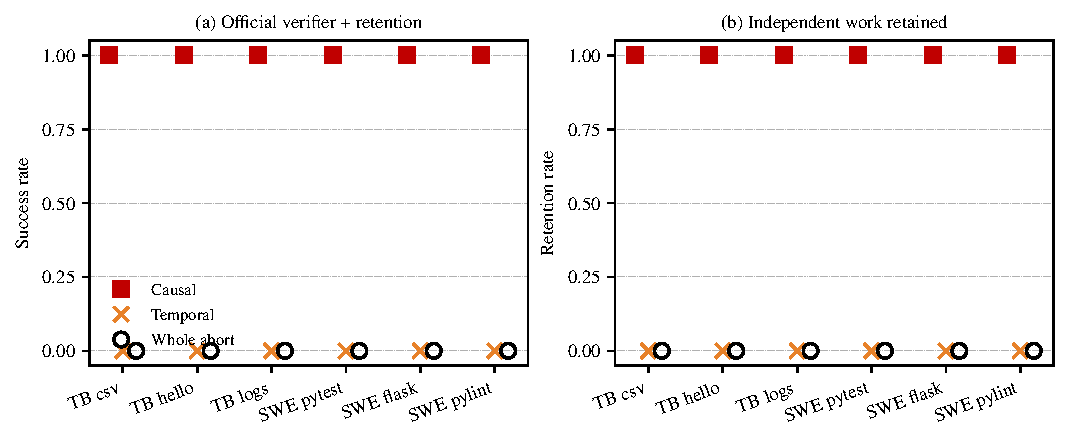
\includegraphics[width=\linewidth]{FIG-Official-Tasks.pdf}
  \caption{\textbf{Official workloads separate recovery from task repair.}
  \small\emph{SWE-Bench Lite and Terminal-Bench, one oracle-repair run per
  cell.  Causal recovery retains independent notes on 6/6 tasks; temporal and
  whole-session abort retain none, while still passing the official verifier.}}
  \label{fig:official-tasks}
\end{figure}

\subsection{RQ5: Failure Recovery and Session Scale}
\label{sec:eval-robust}

We hypothesize that persistent workers, session reload, and the commit WAL
preserve transaction invariants under the tested failures.  The robustness
bundle kills one persistent worker, reloads a 256-step session at step 128, and
runs four agents with 16 writes each.  Figure~\ref{fig:robust} summarizes these
tests.  The killed worker falls back to one-shot \trycmd for the current request
and restarts before the next.  The reloaded session commits all 256 files with
step p50/p95 of 36.3/72.3~ms.  All four agents commit disjoint subtrees without
cross-contamination in 3.105~s.

\begin{figure}[t]
  \centering
  
\includegraphics[width=\linewidth]{FIG-Robustness.pdf}
  \caption{\textbf{The optimized runtime preserves tested invariants.}
  \small\emph{Worker fallback, a 256-step reload, and four disjoint agents all
  complete without losing committed files or contaminating another workspace.}}
  \label{fig:robust}
\end{figure}

Table~\ref{tab:wal} then injects five crashes at each publication phase.
Crashes before a durable frontier restore the pre-image and allow a clean
recommit.  A crash after materialization but before frontier persistence
converges on reload.  A crash during committed cleanup leaves a durable frontier
that reload finalizes.  Unrelated host files remain intact in every cell
(5/5 per phase).

\begin{table}[t]
\centering
\caption{\textbf{WAL phase fault injection.}
\small\emph{Five crashes per phase; recovery is host/frontier convergence after
reload.}}
\label{tab:wal}
\scriptsize
\begin{tabular}{lcc}
\toprule
Phase & Expected outcome & Recovery \\
\midrule
Before prepare & no WAL; recommit & 5/5 \\
Prepared & restore then recommit & 5/5 \\
Applying & restore then recommit & 5/5 \\
During install & restore then recommit & 5/5 \\
Materialized & converge / finalize & 5/5 \\
Committed cleanup & durable frontier & 5/5 \\
\bottomrule
\end{tabular}
\end{table}

The worker and reload tests exercise recovery within one session.  The
concurrency test uses separate workspace subtrees and does not fence concurrent
writes to the same path.  RQ5 therefore validates the tested failure and
isolation cases, not arbitrary overlapping multi-agent publication.

\section{Discussion and Limitations}

\textbf{Why not make causal rollback the default?}
The active view uses OverlayFS \texttt{index=on}, which preserves hard-link
visibility within the tested session~\cite{overlayfs}.  Alias-complete
publication covers complete host-visible groups, tested upper-created groups,
and intentional rename-over replacement.  Causal recovery still fails closed
for arbitrary multi-object topology, bind mounts, external aliases, and
unsupported generation changes.

\textbf{Why trace instead of infer commands?}
Command strings are not a reliable specification of transitive compiler, test,
or script reads.  System-call tracing observes actual accesses but adds
workload-dependent cost and remains Linux-specific.  We therefore use the
strace path for the main correctness and performance claims: in the measured
12-step comparison it costs 25.60 ms/step, versus 61.39 ms/step for the
optional persistent eBPF backend, while both capture the same read and negative
lookup cases in this probe.  The eBPF path remains a replaceable implementation,
not a claim of lower overhead.  Neither tracer removes the need to define alias
and unsupported-syscall semantics or repairs an inode relation already split by
OverlayFS copy-up.

\textbf{What state is outside the transaction?}
The current \aet covers workspace-local filesystem effects.  Network requests,
emails, package registries, cloud control planes, process memory, and terminal
state may be irreversible or require subsystem-specific compensation.  Systems
that capture full process/session state are complementary, not dominated by
\system.

\textbf{Is commit atomic?}
The WAL guarantees deterministic recovery of the session and host after an
interrupted commit.  It does not provide kernel-level all-path atomic visibility
to external observers during materialization.  Workloads requiring that
property need a rename-based publication protocol or a transactional substrate.

\textbf{How strong is the current evidence?}
Deterministic microbenchmarks cover up to 256 steps and controlled DAGs up to 64 calls.
Application evaluation uses SWE-Bench Lite and Terminal-Bench with oracle repair
after recovery; live-agent control-plane runs remain seeded and use one model.
Several recent external systems cannot run on the current VM because of FUSE, CRIU,
kernel, compiler, or privilege requirements.

\section{Related Work}

AgentTX is closest to effect-capturing semisolates, agent-oriented filesystems,
and checkpoint or branch runtimes.  Its distinguishing recovery unit is a
non-contiguous causal subgraph within one speculative trajectory.  We compare
that semantic choice below; without artifact-native measurements, we do not
claim end-to-end superiority.

\textbf{Effect capture and semisolates.}
\trycmd introduces unprivileged semisolates for opaque commands, including
effect introspection, optional application, and stacking~\cite{try-osdi26}.
\system uses these mechanisms as its execution substrate.  Its focus is the
long-lived trajectory: automatic cross-step dependencies, non-contiguous causal
recovery, frontier materialization, policy persistence, and commit WAL.

\textbf{Agent-native filesystems and branches.}
YoloFS stages mutations, exposes snapshots, and uses progressive permission to
improve agent/user control~\cite{yolofs}.  Its filesystem mediation and
permission interface are broader than \system's current substrate.  BranchFS
provides nested copy-on-write branch contexts with atomic leaf commit/abort and
first-commit-wins coordination~\cite{branchfs}.  These systems select snapshots
or branches; \system selects a causal subgraph inside one evolving trajectory.

\textbf{Checkpoint and restore.}
Waypoint combines filesystem deltas with process, memory, shell, and terminal
state for branchable sessions~\cite{waypoint}.  DeltaBox accelerates complete
sandbox checkpoint/rollback using incremental filesystem and process
state~\cite{deltabox}.  Crab observes turn-level effects to avoid checkpoints
that do not contain recovery-relevant state~\cite{crab}.  Their state coverage
or checkpoint efficiency is complementary to \system.  \system instead answers
which non-contiguous filesystem effects to remove after a failure has been
identified.

\textbf{Process checkpointing and file transactions.}
CRIU and DMTCP preserve complete process/session state for restart, migration,
or debugging~\cite{criu,dmtcp}; their recovery unit is an application image,
not a selected filesystem effect subgraph.  Valor exports POSIX-like file
transactions with kernel logging and locking, while TxFS builds ACID file
transactions on filesystem journaling~\cite{valor,txfs}.  These systems target
atomic publication and crash consistency for explicit transactions.  AgentTX
instead keeps the existing unmodified application interface, infers effects at
opaque tool boundaries, and preserves valid later work after a selective
failure.

\textbf{Filesystem topology and tracing.}
OverlayFS specifies copy-up, whiteout, and index semantics that determine when
two pathnames still denote one object~\cite{overlayfs}.  System-call tracers
such as \texttt{strace} observe accesses made by arbitrary descendants
~\cite{strace}.  The resulting paths still need hierarchy, descriptor, and alias
normalization.
Our contribution is to connect that observation layer to a causal ledger and a
fail-closed reconstruction policy; we do not claim that a different tracer by
itself solves object identity or selective publication.

The surrounding systems literature exposes complementary boundaries.  MicroVM
and userspace-kernel sandboxes study isolation cost~\cite{firecracker,gvisorcase},
while provenance systems record whole-system data and control flow~\cite{camflow}.
Kernel tracing work uses eBPF for low-overhead event capture and distributed
path reconstruction~\cite{ebpfruntime,nahida}.  Storage-oriented
crash-consistency and snapshot systems provide complementary durability
mechanisms, but they recover at a storage or checkpoint boundary rather than
at the causal effect boundary studied here.

\section{Conclusion}

Long-running coding agents need a transaction boundary larger than one command
and a recovery unit smaller than one session.  An Agent Effect Transaction
selects a causal subgraph of versioned effects instead of a temporal suffix.
\system realizes this abstraction with shared speculation, an effect ledger,
selective reconstruction, and a durable commit frontier.  In 144 controlled
runs, it retained all independent work and removed all invalid descendants; at
48 document entries, it also avoided measurable LLM replay.  The result is
limited to supported workspace-local filesystem effects and fail-closed object
identity.

\bibliographystyle{unsrt}
\normalsize
\bibliography{references}

\end{document}
